\begin{question}[ID=1.1, subtitle={Proiettile a 60° — tempo di volo e gittata}, tags={moto parabolico, gittata}, difficulty=facile]
Un cacciatore spara un proiettile alla velocità di $300\ \mathrm{m/s}$ con angolazione di $60^\circ$ rispetto al suolo. Senza attrito dell'aria:
\begin{enumerate}
\item Calcolare il tempo di volo del proiettile.
\item Calcolare la gittata.
\item Calcolare la gittata con angolo $30^\circ$.
\end{enumerate}

\begin{solution}
Nel moto parabolico il moto orizzontale è uniforme e quello verticale è uniformemente accelerato: i due si studiano separatamente.
\begin{enumerate}
\item Il tempo di volo si ricava dal moto verticale: il proiettile torna alla quota di partenza quando la velocità verticale ha invertito completamente il segno. Con $v_{0y} = 300\sin 60^\circ = 259{,}8\ \mathrm{m/s}$:
\[
t = \frac{2v_{0y}}{g} = \frac{2\cdot 259{,}8}{9{,}81} \approx \mathbf{53{,}0\ \mathrm{s}}.
\]
\item La gittata è lo spazio percorso orizzontalmente in questo tempo; usando la formula compatta $R = v_0^2\sin(2\theta)/g$:
\[
R = \frac{v_0^2\sin(2\cdot 60^\circ)}{g} = \frac{300^2\cdot\sin 120^\circ}{9{,}81} \approx \mathbf{7954\ \mathrm{m}}.
\]
\item Poiché $\sin(2\cdot 30^\circ) = \sin 60^\circ = \sin 120^\circ$, la gittata a $30^\circ$ è \textbf{identica} a quella a $60^\circ$: angoli complementari danno la stessa gittata.
\end{enumerate}
\end{solution}
\end{question}

%------------------------------------------------------------------------------------%

\begin{question}[ID=1.2, subtitle={Caduta da aereo in volo orizzontale}, tags={moto parabolico, caduta libera}, difficulty=facile]
Un aereo vola orizzontalmente a $500\ \mathrm{km/h}$ a una quota di $1000\ \mathrm{m}$. Da esso viene lasciato cadere un oggetto.
\begin{enumerate}
\item Calcola il tempo di caduta.
\item Calcola la distanza orizzontale percorsa durante la caduta.
\end{enumerate}

\begin{solution}
\begin{enumerate}
\item Il tempo di caduta dipende solo dal moto verticale, che è una caduta libera da fermo (la velocità iniziale è orizzontale). Da $h = \tfrac{1}{2}gt^2$:
\[
t = \sqrt{\frac{2h}{g}} = \sqrt{\frac{2000}{9{,}81}} \approx \mathbf{14{,}3\ \mathrm{s}}.
\]
\item Orizzontalmente l'oggetto mantiene la velocità dell'aereo (moto uniforme). Convertendo $500\ \mathrm{km/h} = 138{,}9\ \mathrm{m/s}$:
\[
x = v_x\,t = 138{,}9\cdot 14{,}3 \approx \mathbf{1986\ \mathrm{m}} \approx 2{,}0\ \mathrm{km}.
\]
\end{enumerate}
\end{solution}
\end{question}

%------------------------------------------------------------------------------------%

\begin{question}[ID=1.3, subtitle={Lancio orizzontale da 10 m di altezza}, tags={moto parabolico, lancio orizzontale}, difficulty=facile]
Una pallina è lanciata orizzontalmente da $h = 10\ \mathrm{m}$ con velocità iniziale $v_0 = 8{,}5\ \mathrm{m/s}$.
\begin{enumerate}
\item Calcola il tempo di caduta.
\item Calcola la gittata.
\end{enumerate}

\begin{solution}
\begin{enumerate}
\item Come in ogni lancio orizzontale, il moto verticale è una caduta libera indipendente dalla velocità iniziale:
\[
t = \sqrt{\frac{2h}{g}} = \sqrt{\frac{20}{9{,}81}} \approx \mathbf{1{,}43\ \mathrm{s}}.
\]
\item La gittata è la distanza orizzontale coperta a velocità costante in quel tempo:
\[
R = v_0\,t = 8{,}5\cdot 1{,}43 \approx \mathbf{12{,}1\ \mathrm{m}}.
\]
\end{enumerate}
\end{solution}
\end{question}

%------------------------------------------------------------------------------------%

\begin{question}[ID=1.4, subtitle={Cannone a 1 m da terra con v₀ = 4 m/s a 30°}, tags={moto parabolico, traiettoria}, difficulty=media]
Un cannone posto a $h_0 = 1\ \mathrm{m}$ spara una palla con $v_0 = 4\ \mathrm{m/s}$ a $30^\circ$ rispetto all'orizzontale.
\begin{enumerate}
\item Determina le componenti della velocità iniziale.
\item Ricava l'equazione della traiettoria.
\item Calcola l'altezza massima raggiunta.
\end{enumerate}

\begin{solution}
\begin{enumerate}
\item Scomponiamo la velocità iniziale lungo gli assi:
\[
v_{0x} = v_0\cos 30^\circ = 3{,}46\ \mathrm{m/s}, \qquad v_{0y} = v_0\sin 30^\circ = 2{,}00\ \mathrm{m/s}.
\]
\item L'equazione della traiettoria si ottiene ricavando $t = x/v_{0x}$ dal moto orizzontale e sostituendolo nella legge oraria verticale $y = h_0 + v_{0y}t - \tfrac{1}{2}gt^2$:
\[
y = 1 + \frac{2{,}00}{3{,}46}\,x - \frac{9{,}81}{2\cdot 3{,}46^2}\,x^2 \approx 1 + 0{,}578\,x - 0{,}410\,x^2.
\]
È una parabola con la concavità verso il basso, come atteso.
\item L'altezza massima si raggiunge quando la velocità verticale si annulla; il dislivello salito è $v_{0y}^2/(2g)$, da sommare alla quota di partenza:
\[
h_{max} = h_0 + \frac{v_{0y}^2}{2g} = 1 + \frac{4}{19{,}62} \approx \mathbf{1{,}20\ \mathrm{m}}.
\]
\end{enumerate}
\end{solution}
\end{question}

%------------------------------------------------------------------------------------%

\begin{question}[ID=1.5, subtitle={Lancio orizzontale: velocità finale doppia della iniziale}, tags={moto parabolico, lancio orizzontale}, difficulty=media]
Una pallina è lanciata orizzontalmente da $h = 12\ \mathrm{m}$; il modulo della velocità al suolo è il doppio della velocità iniziale. Determina la velocità iniziale.

\begin{solution}
Al suolo la velocità ha due componenti: quella orizzontale resta $v_x = v_0$, mentre quella verticale è quella acquisita nella caduta libera:
\[
v_y = \sqrt{2gh} = \sqrt{2\cdot 9{,}81\cdot 12} = 15{,}34\ \mathrm{m/s}.
\]
Imponiamo la condizione che la velocità finale (modulo) sia doppia di quella iniziale, $\sqrt{v_0^2 + v_y^2} = 2v_0$, ed eleviamo al quadrato:
\[
v_0^2 + 235{,}4 = 4v_0^2 \;\Rightarrow\; v_0 = \sqrt{\frac{235{,}4}{3}} \approx \mathbf{8{,}86\ \mathrm{m/s}}.
\]
\end{solution}
\end{question}

%------------------------------------------------------------------------------------%

\begin{question}[ID=1.6, subtitle={Sacchetto di sabbia lanciato sopra un muro}, tags={moto parabolico}, difficulty=media]
\begin{minipage}{\linewidth}
\begin{wrapfigure}{r}{0.25\textwidth}
    \centering
    \vspace{-30pt}
    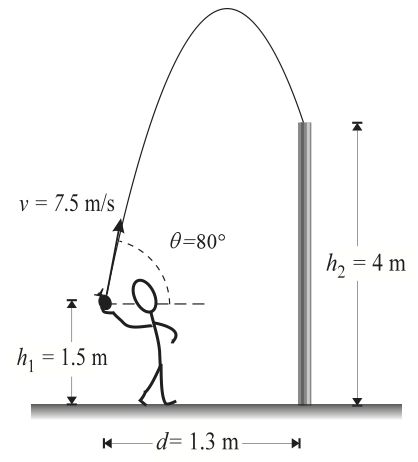
\includegraphics[width=0.25\textwidth]{images/sacchetto_moto_parabolico.jpg}
\end{wrapfigure}
Un ragazzo lancia un sacchetto di sabbia sopra un muro alto $4\ \mathrm{m}$ posto a $1{,}3\ \mathrm{m}$ davanti a lui. Il sacchetto si stacca a $h_0 = 1{,}5\ \mathrm{m}$ da terra con $v_0 = 7{,}5\ \mathrm{m/s}$ a $80^\circ$ dall'orizzontale.

Quanto dura il volo del sacchetto?
\end{minipage}
\begin{solution}
Scomponiamo la velocità iniziale:
\[
v_{0x} = 7{,}5\cos 80^\circ = 1{,}302\ \mathrm{m/s}, \qquad v_{0y} = 7{,}5\sin 80^\circ = 7{,}386\ \mathrm{m/s}.
\]
Verifichiamo innanzitutto che il sacchetto superi il muro. Esso raggiunge l'ascissa del muro ($x = 1{,}3\ \mathrm{m}$) all'istante $t_1 = 1{,}3/1{,}302 \approx 1{,}0\ \mathrm{s}$, a una quota
\[
y(t_1) = 1{,}5 + 7{,}386\cdot 1 - \tfrac{1}{2}\cdot 9{,}81\cdot 1^2 \approx 3{,}99\ \mathrm{m} \approx 4\ \mathrm{m},
\]
quindi passa appena sopra il muro. La durata totale del volo si trova imponendo il ritorno a terra ($y = 0$):
\[
1{,}5 + 7{,}386\,t - 4{,}905\,t^2 = 0 \;\Rightarrow\; t \approx \mathbf{1{,}68\ \mathrm{s}},
\]
prendendo la soluzione positiva dell'equazione di secondo grado.
\end{solution}
\end{question}

%------------------------------------------------------------------------------------%

\begin{question}[ID=1.7, subtitle={David e Golia: velocità e frequenza della fionda}, tags={moto parabolico, moto circolare, traiettoria}, difficulty=difficile]
David lancia un sasso con la fionda a $45^\circ$ dall'altezza $h_0 = 70\ \mathrm{cm}$. L'occhio di Golia è a $H = 1{,}80\ \mathrm{m}$ dal suolo e a distanza orizzontale $d = 12\ \mathrm{m}$.
\begin{enumerate}[parsep=0pt,itemsep=2pt]
    \item Determina la velocità di lancio affinché il sasso colpisca l'occhio di Golia.
    \item Determina la frequenza di rotazione della fionda (raggio $r = 20\ \mathrm{cm}$).
\end{enumerate}
\begin{solution}
\begin{enumerate}
    \item Con $\theta = 45^\circ$ le componenti sono uguali, $v_{0x} = v_{0y} = v_0/\sqrt{2}$. Dal moto orizzontale ricaviamo il tempo per raggiungere Golia:
    \[
    d = v_{0x}\,t \;\Rightarrow\; t = \frac{d\sqrt{2}}{v_0} = \frac{12\sqrt{2}}{v_0}.
    \]
    Sostituiamo nella legge oraria verticale imponendo $y = H$ all'arrivo:
    \[
    H = h_0 + v_{0y}t - \tfrac{1}{2}gt^2 \;\Rightarrow\; 1{,}80 = 0{,}70 + \frac{v_0}{\sqrt{2}}\cdot\frac{12\sqrt{2}}{v_0} - \frac{g}{2}\cdot\frac{288}{v_0^2}.
    \]
    Il termine lineare si semplifica e l'equazione si risolve rispetto a $v_0^2$:
    \[
    1{,}10 = 12 - \frac{1413{,}4}{v_0^2} \;\Rightarrow\; v_0^2 = \frac{1413{,}4}{10{,}90} \approx 129{,}7 \;\Rightarrow\; v_0 \approx \mathbf{11{,}4\ \mathrm{m/s}}.
    \]
    \item La velocità di lancio è la velocità tangenziale che la fionda imprime al sasso, $v_0 = \omega r = 2\pi f\,r$. Ricavando la frequenza:
    \[
    f = \frac{v_0}{2\pi r} = \frac{11{,}4}{2\pi\cdot 0{,}20} \approx \mathbf{9{,}07\ \mathrm{Hz}}.
    \]
\end{enumerate}
\end{solution}
\end{question}
